Studiamo adesso in dettaglio il legame chimico.

Prima di addentrarci nell'argomento però, bisogna notare che esistono speci chimiche di cui non esiste la molecola, ma solo il solido: i composti ionici. Un esempio di tali composti è l'NaCl: la specie molecolare del cloruro di sodio non esiste, ma esiste il solido.

Dobbiamo allora comprendere perché non esistono le molecole singole delle speci fortemente ioniche, per poi ragionare sul legame chimico, che ha una natura diversa nei sistemi molecolari.

Dobbiamo quindi rispondere a una serie di domande:
\begin{itemize}
    \item Perché si formano le molecole, dato che molti sistemi non esistono come tali?
    \item Quali condizioni bisogna soddisfare affinché il composto che si forma a seguito di una reazione, sia stabile?
    \item Perché esistono geometrie ben definite?
\end{itemize}
Prima di andare avanti va da ricordare che, in linea generale, se facciamo reagire una specie A con una specie B otterremo una specie C in modo spontaneo solo se l'energia del sistema diminuisce. 

Ricordiamo poi che qualunque stato legato avrà un'energia potenziale negativa: in un sistema AB dove A e B sono due atomi, essi sono legati se la loro energia potenziale è minore di zero. Se per qualche motivo l'energia dovesse aumentare, nell'istante in cui essa diventasse pari a zero gli atomi non sarebbero più legati.

Ragioniamo solo sull'energia potenziale per via dell'esistenza del teorema del viriale, il quale afferma che

\vspace{0.2cm}"\textit{La variazione dell'energia totale di un sistema ha lo stesso segno della variazione dell'energia potenziale}"

\vspace{0.2cm}Quindi la molecola AB si formerà nel momento in cui l'energia potenziale dei due atomi A e B diminuisce (fino a diventare negativa) man mano che li avviciniamo.

\vspace{0.2cm}Per una molecola o un sistema di pochi atomi siamo in grado di fare ragionamenti estremamente sofisticati anche se non riusciamo a risolvere con esattezza l'equazione di Schrödinger, ma solo in maniera ragionevolmente approssimata, nel senso che le soluzioni ottenute non si discostano molto da valori che si ottengono sperimentalmente, ossia la descrizione approssimata risulta essere estremamente accurata per le capacità di calcolo e di modellizzazione ad oggi a disposizione.

Per essi si usa la teoria degli orbitali molecolari, che vedremo dopo.

Nell'istante in cui invece i sistemi che indaghiamo diventano complessi (molti atomi, molecole grandi con elevati pesi molecolari), non siamo più in grado, solo per esigenze di calcolo, di ottenere soluzioni approssimate ragionevolmente.

Per essi allora bisogna usare una catalogazione precedente, che si basava sul tipo di legame presente tra le molecole in esame.
Un parametro estremamente utile a comprendere i sistemi è il concetto di elettronegatività, che è la tendenza che hanno i diversi atomi ad attrarre su di sé la carica di legame. Nel momento in cui uno dei due atomi costituenti il nucleo è abbastanza più elettronegativo dell'altro, si avrà una dislocazione della carica di legame, per cui diremo che la molecola avrà una sua polarità, ossia mostrerà una parziale carica positiva e una parziale carica negativa, la quale nei fatti costituisce un dipolo.

In base al valore della differenza di elettronegatività, il legame verrà etichettato in vari modi:
\begin{itemize}
    \item Se è piccola (fino a 0.4) si parla di \textbf{legame covalente};
    \item Se inizia a crescere ma è comunque contenuta (da 0.4 fino a 1.9) si parla di \textbf{legame} covalente \textbf{polare}, e la molecola avrà una polarità cospicua. 
    \item Se diventa molto grande (da 1.9 in poi) si parla di \textbf{legame ionico}.
\end{itemize} 

\subsection{Il legame polare}
In questo caso ci saranno parziali cariche positive e negative, che possono venire indicate in diversi modi: o rispettivamente con $\delta^+$ e $\delta^-$, o con zone rosse e blu che indicano rispettivamente addensamento di elettroni e le zone che si sono positivizzate, o con una freccia con la punta e una croce, dove la punta è rivolta verso l'atomo più elettronegativo.

\subsection{Il legame metallico}
È necessario fare un discorso a parte per i sistemi metallici. Per essi è possibile immaginare che gli elettroni siano abbastanza liberi, nel senso che rispetto ai legami visti in precedenza gli elettroni sono legati pochissimo all'atomo, tanto da essere considerati come un gas che statisticamente neutralizza i nuclei, il quale viene detto \textit{mare di elettroni}.

\begin{figure}[htp]
    \centering
    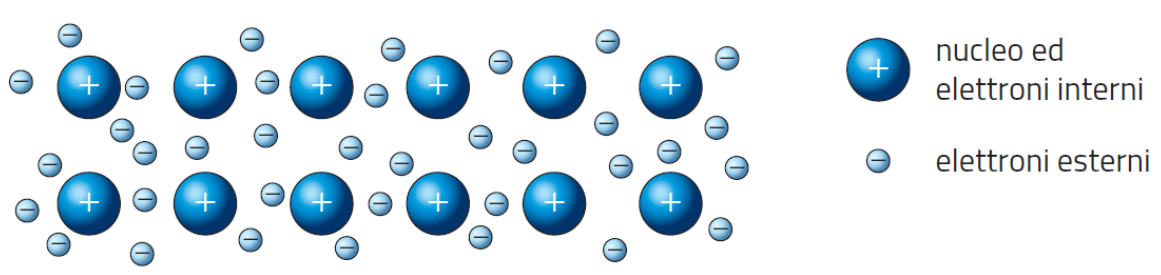
\includegraphics[width=14cm]{immagini/legame-metallico.png}
\end{figure}

Nei metalli gli atomi occupano posizioni ben definite all'interno di una struttura cristallina. A differenza dei composti ionici, però, qua non possiamo parlare di ioni: gli atomi sono neutri, solo che i loro elettroni esterni occupano una banda e non più un livello. Finora infatti abbiamo parlato di energie ben precise per gli orbitali, ma non è più così all'interno di una banda, o per meglio dire l'energia dei singoli livelli continua ad esserci, ma poiché essi sono in numero elevato, possiamo immaginare che la differenza in energia tra un livello energetico e il successivo sia piccolissima, al punto tale da immaginare non più l'esistenza di orbitali con energie nette e separate, ma una banda all'interno della quale l'elettrone possa muoversi.

\subsection{Esempi vari}
Nei vari esempi che seguono, per razionalizzare i valori sperimentali dei momenti di dipolo, ragioneremo sulla direzionalità dei legami e sulla differenza di elettronegatività degli atomi coinvolti.

\vspace{0.2cm}\textbf{ES.1} F$_2$

\vspace{-0.3cm}\begin{figure}[H]
    \centering
    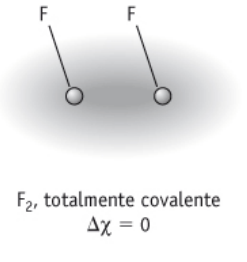
\includegraphics[width=5cm]{immagini/F_2.png}
\end{figure}

\vspace{-0.7cm}Due atomi di fluoro formano la molecola F$_2$. Sebbene il fluoro sia estremamente elettronegativo, i due atomi sono uguali, per cui la differenza in elettronegatività è pari a zero, quindi la condivisione dei due elettroni di legame è totale e il sistema è covalente.

\vspace{0.2cm}\textbf{ES.2} HF

\vspace{-0.3cm}\begin{figure}[H]
    \centering
    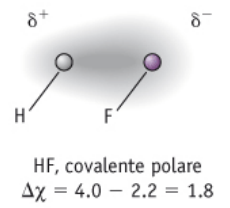
\includegraphics[width=4.8cm]{immagini/HF.png}
\end{figure}

\vspace{-0.4cm}Nell'acido fluoridrico la differenza di elettronegatività tra i due atomi è cospicua, e infatti la carica di legame(che può essere immaginata come una nube elettronica che circonda i due atomi) sarà più spostata verso l'atomo di fluoro e quindi meno presente sull'idrogeno. Il legame sarà allora covalente polare, con una parziale carica negativa $\delta^-$ sul fluoro e una parziale carica positiva $\delta^+$ sull'idrogeno. 

\vspace{0.2cm}\textbf{ES.3} LiF

\vspace{-0.3cm}\begin{figure}[H]
    \centering
    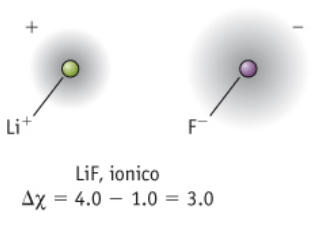
\includegraphics[width=6.4cm]{immagini/LiF.png}
\end{figure}

\vspace{-0.8cm}In un sistema come il fluoruro di litio, la differenza di elettronegatività è elevata, per cui non ci sarà la nube continua tra i due atomi.

Per questi sistemi si immagina che si abbia una cessione di elettroni, per cui non avremo Li e F ma Li$^+$ e F$^-$, cioè è come se il litio avesse ceduto il suo elettrone di valenza al fluoro, il quale tra l'altro acquistandolo avrà configurazione elettronica esterna tipo gas nobile.

Un sistema siffatto è etichettato sistema ionico.

\vspace{0.2cm}\textbf{ES.4} HCl

\vspace{-0.4cm}\begin{figure}[htp]
    \centering
    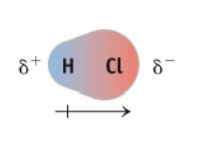
\includegraphics[width=6cm]{immagini/HCl.png}
\end{figure}

\vspace{-0.4cm}Nell'acido cloridrico la differenza di elettronegatività tra idrogeno e cloro è abbastanza evidente, per cui il legame è covalente polare.

Dato che stiamo ipotizzando che su tale molecola ci sia una buona polarità, come conseguenza ci aspettiamo un momento di dipolo.
Per verificarne l'esistenza basta mettere dell'HCl gassoso in un contenitore dove sono presenti le espansioni polari di un elettromagnete. Se il campo elettrico è nullo, l'orientazione delle molecole sarà casuale, se invece applichiamo una differenza di potenziale tra le due piastre osserveremo che le molecole si orientano in modo tale che il cloro sia rivolto verso la lamina positiva (a potenziale maggiore).
\begin{figure}[htp]
    \centering
    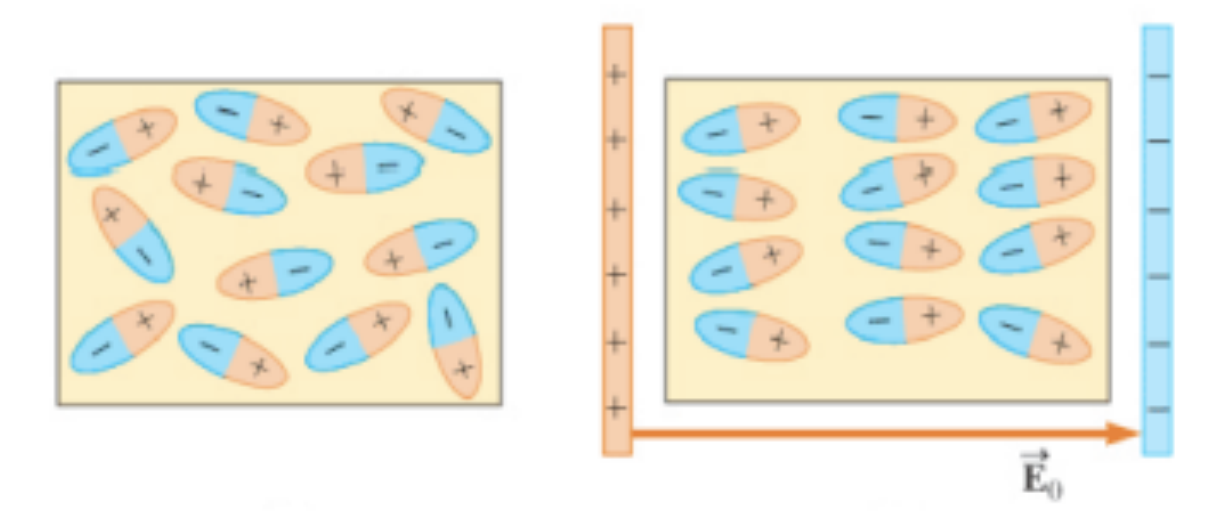
\includegraphics[width=12cm]{immagini/condensatore.png}
\end{figure}
Come facciamo ad accorgercene?
Il sistema che si viene così a costituire è un condensatore, dove tra le armature anziché il vuoto c'è un dielettrico: l'HCl. In questo modo possiamo quindi misurare il momento di dipolo, la cui unità di misura nel SI è il Coulomb per metro, con cui le molecole danno dei valori dell'ordine di 10$^{-30}$, per cui si usa un'altra unità di misura che è il Debye (D). Vale la relazione:
$$1D=3.336\cdot10^{-30}$$
Per l'acido cloridrico si misura un momento di dipolo pari a 1.03 D.
\newpage
\vspace{0.2cm}\textbf{ES.5} CO$_2$

\hspace{0.5cm}\begin{minipage}{0.2\textwidth}
    \begin{figure}[H]
    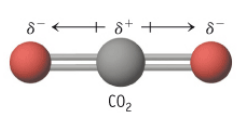
\includegraphics[width=4cm]{immagini/CO_2.png}
    \end{figure}
    \end{minipage} \hfill
    \begin{minipage}{0.65\textwidth}
    \vspace{0.4cm}Descrivendo l'anidride carbonica col formalismo di Lewis notavamo che sul carbonio non ci sono coppie solitarie, perché raggiunge l'ottetto grazie ai due doppi legami carbonio-ossigeno, mentre su ciascun ossigeno ce ne sono due. La geometria che tiene più lontani i due atomi di ossigeno con le coppie di elettroni rimaste è quella lineare.
    
    La differenza in elettronegatività tra carbonio e ossigeno è cospicua, quindi singolarmente troviamo un momento di dipolo nei due diversi legami, ma questi si annullano a vicenda perché sono uguali in modulo ma opposti in verso. Pertanto questa molecola ha un momento di dipolo netto pari a zero, cioè non è polare, pur essendo polari i singoli legami.
    \end{minipage}

\vspace{0.2cm}\textbf{ES.6} H$_2$O

\hspace{0.5cm}\begin{minipage}{0.2\textwidth}
    \begin{figure}[H]
    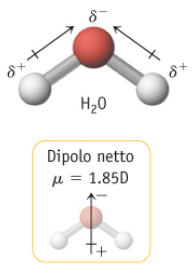
\includegraphics[width=3cm]{immagini/H_2O.png}
    \end{figure}
    \end{minipage} \hfill
    \begin{minipage}{0.65\textwidth}
    \vspace{0.6cm}Descrivendo l'acqua col formalismo di Lewis notavamo due coppie solitarie sull'ossigeno. Dovendo ragionare su un sistema con 4 coppie di elettroni usiamo l'idea del sistema tetraedrico nel quale però le due coppie solitarie stringono il legame, che avrà un angolo di 104.5°. Considerando solo gli atomi, questa molecola sarà piana ma angolata.

    La differenza in elettronegatività tra idrogeno e ossigeno è cospicua, per cui entrambi i legami mostreranno un momento di dipolo. In questo caso però, a causa della geometria molecolare, la loro composizione dà luogo ad un momento di dipolo netto pari a 1.85 D. Grazie ad esso l'acqua è la molecola che permette la vita.    
    \end{minipage}

\vspace{0.2cm}\textbf{ES.7} BF$_3$

\begin{figure}[htp]
    \centering
    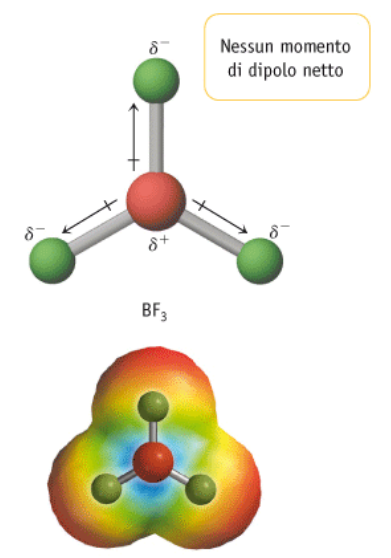
\includegraphics[width=10cm]{immagini/BF_3-dipolo.png}
\end{figure}

Nel descrivere tale molecola abbiamo detto che il boro presenta ibridizzazione sp$^2$, per cui essa sarà una molecola planare con angoli di 120°.

Il fluoro è parecchio più elettronegativo del boro, quindi ciascun legame mostrerà polarità, con la carica di legame addensata sul fluoro.

Essendo planare, la composizione dei tre momenti di dipolo, fra loro uguali in modulo, dà un momento di dipolo netto pari a zero, per cui il BF$_3$ non ha polarità. 
\newpage
\vspace{0.2cm}\textbf{ES.8} Cl$_2$CO

\vspace{-0.3cm}\begin{figure}[htp]
    \centering
    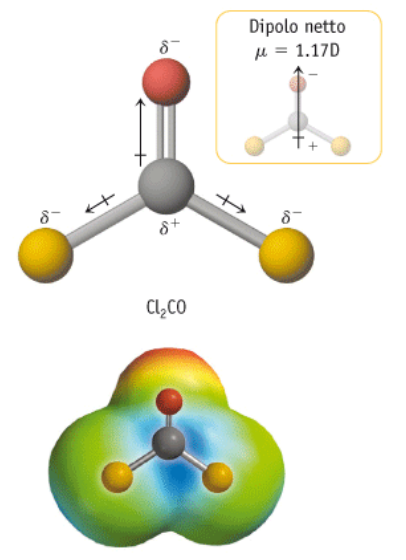
\includegraphics[width=10cm]{immagini/Cl_2CO.png}
\end{figure}

\vspace{-0.3cm}Nel fosgene un atomo di carbonio centrale è legato all'ossigeno tramite un doppio legame e a due atomi di cloro tramite due legami semplici. Sia il cloro che l'ossigeno sono parecchio più elettronegativi del carbonio, quindi ciascun legame mostrerà polarità con la freccia rivolta verso gli atomi esterni. Il momento di dipolo del legame carbonio-ossigeno è più forte, per cui la composizione darà un momento di dipolo netto pari a 1.17 D.

\vspace{0.2cm}\textbf{ES.9} NH$_3$

\vspace{-0.3cm}\begin{figure}[htp]
    \centering
    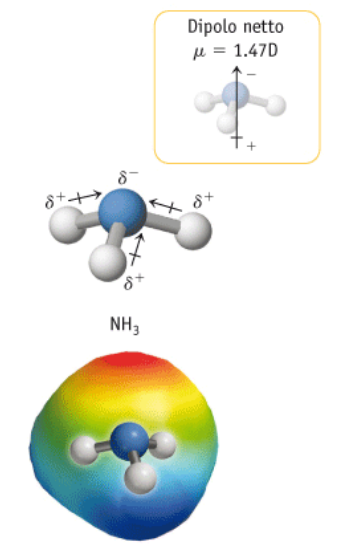
\includegraphics[width=10cm]{immagini/NH_3.png}
\end{figure}

\vspace{-0.3cm}Nell'ammoniaca è l'azoto centrale ad essere più elettronegativo, e lo è parecchio rispetto all'idrogeno. Ne segue che ogni legame mostrerà una polarità la cui freccia è rivolta verso questo. Inoltre col formalismo di Lewis abbiamo visto che su di esso è presente una coppia solitaria, la quale lo solleva dal piano dei tre atomi di idrogeno, per cui il momento di dipolo netto sarà diverso da zero.

Se non ci fosse stata la coppia solitaria, l'azoto si sarebbe disposto nel piano individuato dai 3 idrogeni come nel caso del $\rm BF_3$ e quindi non si avrebbe avuto un momento di dipolo netto.

\vspace{0.2cm}\textbf{ES.10} CH$_4$

\hspace{0.5cm}\begin{minipage}{0.2\textwidth}
\begin{figure}[H]
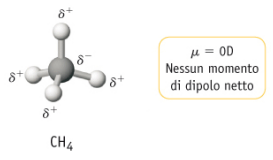
\includegraphics[width=5cm]{immagini/CH_4.png}
\end{figure}
\end{minipage} \hfill
\begin{minipage}{0.5\textwidth}
 Nel metano c'è una buona differenza in elettronegatività tra carbonio e idrogeno, ma a causa della sua geometria tetraedrica la risultante dei momenti di dipolo, uno per ciascun legame, è pari a zero. Nei fatti non si osserva alcun momento di dipolo.
\end{minipage}

\vspace{0.2cm}\textbf{ES.11} CH$_3$Cl (cloroformio)

\hspace{0.5cm}\begin{minipage}{0.2\textwidth}
\begin{figure}[H]
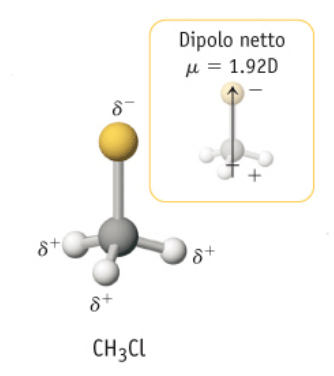
\includegraphics[width=5cm]{immagini/CH_3Cl.png}
\end{figure}
\end{minipage} \hfill
\begin{minipage}{0.5\textwidth}
\vspace{0.4cm}Se nel metano sostituiamo un idrogeno qualunque con un atomo di cloro, la molecola così ottenuta mostra un momento di dipolo netto. Il motivo è che il momento di dipolo del legame cloro-carbonio non è più equivalente agli altri tre, per cui nella loro composizione non si annullano a vicenda.
\end{minipage}
\newpage
\vspace{0.2cm}\textbf{ES.12} CH$_2$Cl$_2$

\hspace{0.5cm}\begin{minipage}{0.2\textwidth}
\begin{figure}[H]
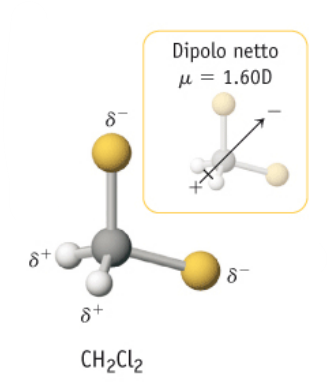
\includegraphics[width=5cm]{immagini/CH_2Cl_2.png}
\end{figure}
\end{minipage} \hfill
\begin{minipage}{0.5\textwidth}
Se sostituiamo un secondo idrogeno con un altro atomo di cloro, la composizione dei momenti di dipolo ne darà uno netto ancora diverso da zero, sebbene minore rispetto al caso precedente.
\end{minipage}

\vspace{0.2cm}\textbf{ES.13} CHCl$_3$

\hspace{0.5cm}\begin{minipage}{0.2\textwidth}
\begin{figure}[H]
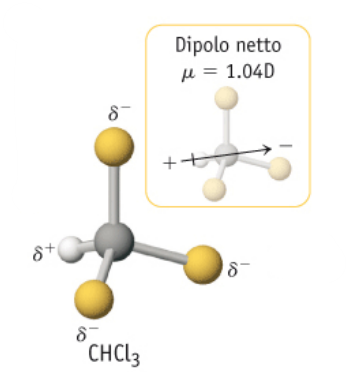
\includegraphics[width=5cm]{immagini/CHCl_3.png}
\end{figure}
\end{minipage} \hfill
\begin{minipage}{0.5\textwidth}
Sostituendo anche un terzo idrogeno con un ulteriore atomo di cloro, la composizione dei momenti di dipolo sarà anche stavolta diversa da zero, ma ancora più piccola.
\end{minipage}

\vspace{0.2cm}\textbf{ES.14} CCl$_4$

\hspace{0.5cm}\begin{minipage}{0.2\textwidth}
\begin{figure}[H]
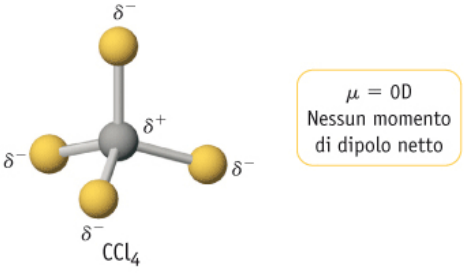
\includegraphics[width=5cm]{immagini/CCl_4.png}
\end{figure}
\end{minipage} \hfill
\begin{minipage}{0.5\textwidth}
Nel momento in cui anche il quarto e ultimo idrogeno viene sostituito con un atomo di cloro otteniamo il tetracloruro di carbonio, il cui sistema sarà di nuovo simmetrico. Per esso la composizione dei momenti di dipolo sarà pari a zero, fatto confermato dalle evidenze sperimentali.
\end{minipage}

\vspace{0.2cm}\textbf{ES.15} L'ordine di legame
\begin{figure}[htp]
    \centering
    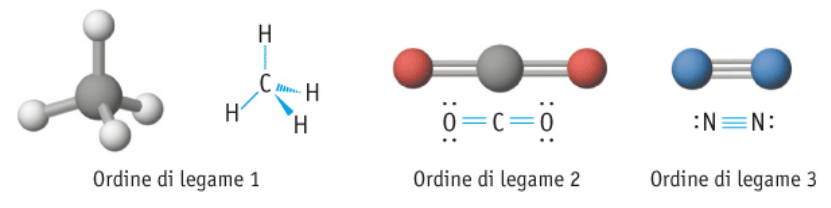
\includegraphics[width=14cm]{immagini/ordine-di-legame.png}
\end{figure}

Consideriamo queste molecole, in modo da dare nuovamente il concetto di ordine di legame. Abbiamo detto che un legame semplice ha ordine di legame 1, uno doppio ordine di legame 2 e uno triplo ordine di legame 3. Tuttavia nell'istante in cui ci fossero sistemi per i quali qualche doppio legame si possa ripartire su più legami semplici l'ordine non era più intero, ma frazionario.


